\chapter{Project Management}
\label{chap:projectManagement}

\begin{table}[t]
	\begin{center}
		\begin{tabular}{|p{4cm}|p{7cm}|p{4cm}|}   
			\hline      
			\bf{Name} & \bf{Email} & \bf{Phone number} \\ 
			\hline
			Esben Aarseth & \href{mailto:esbena@stud.ntnu.no}{esbena@stud.ntnu.no} & 48062321   \\     
			\hline
			Aleksander Gisvold & \href{mailto:aleksg@stud.ntnu.no}{aleksg@stud.ntnu.no}
			& 46692443 \\
			\hline
			Jørgen Aaberg & \href{mailto:jorgeaab@stud.ntnu.no}{jorgeaab@stud.ntnu.no} &
			98866209 \\
			\hline
			Eirik Skjeggestad Dale & \href{mailto:eiriksd@stud.ntnu.no}{eiriksd@stud.ntnu.no}
			& 90138539\\
			\hline
			Yngve Svalestuen & \href{mailto:yngvesva@stud.ntnu.no}{yngvesva@stud.ntnu.no} & 99101640 \\
			\hline
		\end{tabular}
		\caption[Members of developer team]{Members of developer team}
		\label{tab:members}
	\end{center}
\end{table}

\section{Members}
Table \ref{tab:members} shows an overview of the names, email addresses and phone numbers
for the members of the developer team.


%\section{Qualities among members}

We have summarized our technical qualities in the following table. Each team member has
evaluated themself.
\begin{table}[h]
\begin{center}
\begin{tabular}{|p{1.2cm}|p{1.3cm}|p{1.6cm}|p{0.9cm}|p{1.3cm}|p{1.4cm}|p{2cm}|p{1.4cm}|p{2cm}|}
\hline
\bf{Name} & \bf{Java} & \bf{Database} & \bf{\LaTeX} & \bf{Scrum} & \bf{GUI} &
\bf{Management} & \bf{Testing} & \bf{Architecture} \\
\hline
\bf{Aleks} & Medium & Low & Low & High &	High &	Medium & Low &	Medium \\
\hline \bf{Esben} & Medium & Medium & Low	& Medium & High	& Medium & Low	& High
\\
\hline \bf{Jørgen} & Medium & Low & Low & Low & High &	Medium & Medium & Medium
\\
\hline \bf{Eirik} & High & Low & Low & Low	& Medium	& Medium	& Medium	& High \\
\hline \bf{Yngve} & High & Low &	Low & Medium & Medium & Low & Medium & Medium
\\
\hline

\end{tabular}
\end{center}
\end{table}


\section{Roles}
Early in the planning phase, on August 24th 2012, the group held a meeting to distribute
team roles for the project. We discussed which parts were needed for a system fitting the description,
and we decided on four main parts: GUI, back-end, database and Karotz. In addition, proper development
requires testing so we saw the need for a person in charge of testing, and a person in charge of
general quality assurance. We also needed a high-level system architect who could keep the
project well-structured and easily maintainable, especially considering that the system spans over
at least three different subsystems (database, Karotz and Android applications). Since the group was to keep
close contact with both the customer and the group advisor, responsibilities were assigned to these
roles as well. There would also be a need to write reports for meetings with these third parties, so
a secretary was necessary. At last, the group had already decided to use an agile 
development model, so a person in charge of this was needed as well (``Scrum master").

We have identified the following roles for the project. 
\begin{itemize}
\item Test Master - Eirik
\item Scrum Master - Aleksander
\item Customer Contact - Aleksander
\item Advisor Contact - Esben
\item Document Owner - Yngve
\item Secretary - Jørgen
\item Karotz Developer - Yngve
\item Database Manager - Yngve
\item System Architect - Esben
\item Quality Assurance manager - Jørgen 
\end{itemize}


\section{Responsibilities among roles}

In the following section all roles and their responsibilities are explained.

\begin{description}
	\item[Test Master] The test master is responsible for developing a test plan, initiate testing 
		and follow up on test results. The test master will have the last vote in 
		whether a test is passed or not. The test master will be responsible for making sure all 
		parts of testing is done, including unit testing, integration testing, system 
		testing and acceptance testing with the customer.
	
	\item[Scrum Master] Scrum master is accountable for removing impediments to the ability of the team 
		to deliver the sprint goal. The scrum master is no team leader, but is a kind 
		of buffer between the development team and distracting influences. The scrum master 
		is responsible for ensuring that the scrum process is 
		used as intended.

	\item[Customer Contact] The customer contact is responsible of all contact with the customer outside 
		of the customer meetings. This includes sending meeting invitations, clarifying 
		questions outside of customer meetings and other inquiries to the customer. 
		The customer contact works as a single-point two-way communicator, to reduce 
		amount of communication points. 

	\item[Advisor Contact] The advisor contact is responsible of all contact with the advisor outside 
		of the advisor meetings. Including sending meeting invitations, clarifying 
		questions outside of advisor meetings and other inquiries to the advisor. Advisor 
		contact works as a single-point two-way communicator, to reduce amount of 
		communication points.

	\item[Document Owner] The Document owner is responsible of finding a suitable tool for writing the report 
		in \LaTeX, and finding solutions with problems regarding \LaTeX. The document owner is also responsible for making sure all the correct 
		documents is added to the report, and will let the group know if something is missing. 

	\item[Secretary]
		Secretary is responsible for taking notes during all internal, 
		customer and advisor meetings. Meeting reports should meet a specific standard, 
		given by the project compendium. It is the responsibility of the meeting 
		report master to ensure this standard is followed.

	\item[Karotz Developer]
		The robot bunny, named Karotz, has an API for implementing features for controlling 
		the robot with an application. 
		The Karotz developer is responsible for developing the Karotz specific part of the system. 

	\item[Database manager]
		The database manager is responsible for selecting a suitable database tool for 
		the applications. The role also includes the responsibility of managing the 
		database architecture and connections towards the database.

	\item[System architect]
		The system architect is responsible of the overall architecture of the source code. 
		The architect has final vote in decisions regarding architecture specific problems. 

	\item[Quality assurance manager]
		The quality assurance manager has the overall responsibility for the applications and reports quality.

\end{description}


\section{Weekly schedule}

The development team had the following fixed weekly schedule:

\begin{itemize}
\item Customer meeting: Monday 12:15-13:00
\item Advisor meeting: Monday 13:15-14:00
\end{itemize}
Rooms were reserved on demand. There were also at least one day a week were the development team works together in the same room. 

\section{Work Plan}
\label{sec:workplan}

\subsection{Phases}

\subsubsection{Planning phase}
In this phase, a lot of time went to researching development methodology,
different useful technologies (like \LaTeX{}, different frameworks, customer
needs, etc.), and deciding upon a template for the software architecture. This phase was scheduled 
for completion by September 16th. 

\subsubsection{Development}
This phase started as soon as the planning phase was completed and
approved by the customer. It included development of the different
applications and testing continuously. This phase was scheduled for completion by
November 15th.

\subsubsection{Report Writing}
This phase included writing the necessary documentation of the final code. A lot of work
was put into writing the report during the development phase. However, as the
report would be large, and we would need the time to make corrections
and add content. This phase was scheduled for completion by November 20th. 

\subsubsection{Planning of presentation}
Planning of the presentation was started after this report was completed. This phase was scheduled
for completion the day before the actual presentation November 22nd. 

\subsection{Activities}
\label{sec:activities}
We identified some big tasks that needed to be done during the project lifetime. These
tasks were essential to make the project a success. 

The identified tasks are:
\begin{itemize}
  \item Workshop
  \item Usability tests
  \item Integration tests
  \item Export applications and wrap up the source code
  \item Project presentation
  \item Final report correction
\end{itemize}

\subsection{Person-hours per activity and phase}
We planned the following person hours per phase. These numbers are based on the estimated project
effort according to the class staff, and how long we thought each phase would take. As the activities identified
in Section \ref{sec:activities} are activities ``baked into'' the different sprints during development, we have not included estimation for these 
(for instance, it is hard to know so early how many usability tests we need). Also, we would write the report continuously, 
and this is considered a subtask of both development and planning. For each sprint we planned to use 175 hours on development.
%TODO: begrunne 175 timer?
\begin{itemize}
  \item Development: 875 hours
  \item Planning: 425 hours
  \item Meetings: 125 hours
  \item Report completion: 30 hours
  \item Presentation planning: 30 hours
\end{itemize}

\subsection{Gantt Diagram}
Figure \ref{fig:gantt} shows the Gantt Diagram for the whole project period.
%TODO: write something about the gantt diagram
\begin{figure}
	\centering
		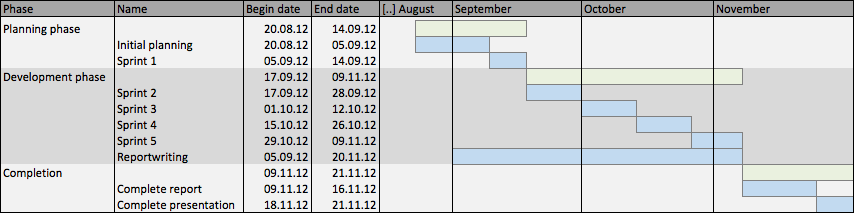
\includegraphics[width = 17.5 cm]{Pictures/ArchPictures/Gantt.png}
	\caption{Gantt project overview}
	\label{fig:gantt}
\end{figure}
\section{Risk Analysis}
This section contains the risk analysis we did before the project was started. The 
analysis helped the team detect the most relevant risks for the project, in order 
to be prepared if such a problem should occur. This allowed the team to make some preemptive 
measures as well as draw up strategies for handling a number of possible situations. 
In addition to a listing of internal and external risks, this section contains a SWOT 
analysis for a deeper understanding of the different relations in the project, both internal and external.

\subsection{Internal Risks}
Table \ref{tab:internalRisks} contains issues that the group identified as possible 
internal risks for the project.

\subsection{External Risks}
Table \ref{tab:externalRisks} contains issues that the group identified as possible external 
risks to the project.

\begin{table}
	\centering
		\begin{sideways}
			\begin{tabular}{|  c 	 |	l 	| 	p{4.0cm} 	 |	p{4.0cm} 	  |	c 	 |	p{4.0cm} 	| 	l| }
			\hline
			  \# & Activity 	& Risk factor 	& Consequences 	& Prob.& Strategy and action 							& Responsible \\
			\hline
			  IR1 & All		& Longterm illness among the development team.  	& M -- Decrease of productivity. Lack of expertise.	& M 	& Share information online. The ill developer keeps himself updated. 	& All \\
			\hline
			  IR2 & All		& Long-term leave. A group member takes a long-term leave.  & M -- Reduced capacity.  & L	&  Plan what the member shall do before he is leaving.		& The Member \\
			\hline
			  IR3 & All		& Internal conflicts among the developer team.		& M -- Bad mood. Less work effort.  & H	&  Bring it up, and handle it right away. Use the advisor. 		& All \\
			\hline
			  IR4 & All		& Deadlines not being reached.			 	& H -- Unfinished work.  & M	&  Predict work load and set project boundaries. 	& Project leader \\
			\hline
			  IR5 & All		& Group members busy with other courses.		 & L -- Reduced capacity & H	&  Common Google Calendar to plan meetings. The member finds another time to do the work. 	& All \\
			\hline
			  IR6 & All		& Group members leaves project.		 	& H -- Reduced capacity & L	&  Reduce the project boundaries.	& All \\
			\hline
			  IR7 & Meetings		& Group members showing up late.	 	& L -- Reduced capacity & H	&  The group member works more next time. Penalties. 	& All \\
			\hline
			  IR8 & Implementation		& Lack of knowledge or abilities.	 	& L -- More time goes to getting knowledge. & M & Getting the knowledge. 	& All \\
			  \hline
			\end{tabular}
		\end{sideways}
	\caption{Internal Risks}
	\label{tab:internalRisks}
\end{table}

\begin{table}
	\centering
		\begin{sideways}
			\begin{tabular}{|  c 	|	p{2.0cm} 	 |	p{4.0cm} 	 |	p{4.0cm} 	  |	c 	 |	p{4.0cm} 	| 	p{2.0cm}| }
				\hline
				  \# & Activity 	& Risk factor 	& Consequences 	& Prob.& Strategy and action 							& Responsible \\
				\hline
				  ER1 & All		& External conflicts. One or more of the group members is in conflict with the customer or the group advisor & M -- May lead to bad communication, lack of feedback etc. & L 	& Bring it up and handle it right away. If customer contact is in a really bad conflict, change customer contact.	& All \\
				\hline
				  ER2 & Design and implementation	& Customer changes requirements. The customer is very decisive and demanding. & H -- May stress the developers and and make them confused on what to prioritize.  & H	&  Force the customer to prioritize tasks. Compromise possible solutions. 	& Development team and customer \\
				\hline
				  ER3 & All		& There is insufficient input from the customer regarding the development process.  & M -- May lead to expectancies not being met.  & L &  Force input from customer.	& Development team and customer \\
				\hline
				  ER4 & Development	& Tools fail. Software tools stop working or are outdated. 	& M -- Development process halted.  & L	&  Do other work. For instance report writing, testing and refactoring. Find other solutions to the problem. & All \\
				\hline
				  ER5 & Development & Loss of data. Data connected to the project is lost, or is unavailable for a period of time.   & H -- Development put back in time. & L &  Prioritize tasks according to remaining time. 	& All \\
				\hline
				  ER6 & Meetings, Feedback	& One of the customers takes a long-term leave. & L -- May delay feedback, input and access to resources. & L & Require more from the other customer contacts. 	& The customer \\
				\hline
				  ER7 & Development & Cannot get the Karotz API to work. & H -- May lead to removal of this feature for the prototype. & L	&  Focus on other parts of the applications.  & Development team \\
				\hline
				  ER8 & Development		& Database not working at all.  & H -- May lead to hardcoding of all features for the prototype. & L & Hardcode necessary parts.	& Development team \\
				\hline
				  ER9 & Development		& Android devices stop working  & L -- May delay development since emulator has low performance. & L & The group member must switch to emulator. 	& Group member \\
				  \hline
			\end{tabular}
		\end{sideways}
	\caption{External Risks}
	\label{tab:externalRisks}
\end{table}

\subsection{SWOT analysis}
The following section contains an analysis of strengths, weaknesses, opportunities and threats 
to the project. The analysis is used as a strategic planning method which analyses the internal 
and external factors in a group. The internal factors are strengths and weaknesses while 
opportunities and threats represent the external factors. 

According to Jackson et. al (2002)\cite{swot}, the SWOT analysis' intended use is to get an overview of the internal and external factors at the 
beginning of the project. Later, the analysis was used to map which parts of the project 
should be relied upon the most, and which opportunities and strengths can help the progress of 
the project the most.
 
Keeping the high-risk parts of the project under close watch helped the team catch problems 
before they evolved. In cases where a diversion was required, the SWOT analysis supported the 
team.
%TODO update references

\subsubsection{Strengths}
Communication and knowledge were the two greatest strengths in the project group. The fact that all 
team members spoke Norwegian as their native language, and were fairly competent in English, made 
all communication and reporting easier. Deciding to do the reporting and programming in English, 
while all other means of communication in Norwegian led to fewer misunderstandings and made 
it easier to help each other out when problems occurred. Discussions were also more valuable 
since everyone were able to participate without the fear of missing out due to lack of understand 
foreign languages.
 
When it comes to the level of knowledge, all group members were fourth year Computer Science students. 
This implied that even though the group members were taking different paths as to which 
specialization they were following for their masters degree, they all had a common background. 
It was therefore to be expected that everyone could participate in both coding and writing. The 
consequences of somebody falling ill were low, since they could be replaced by another member of 
the team. 

The technology was being shared between all team members and every team member took part in each part of the development. 
In addition to the basic knowledge, team members have chosen their own combination of courses. 
This made the team more capable of solving a broad array of tasks and finding good solutions to problems. 
Another strength in the group was that everyone had experience from previous projects, some more 
than others, but everyone had been involved in IT related projects. This provided the team with 
the experience needed to avoid some common pitfalls and get a decent start on the projects. 
The applications is to be used by patients with chronic illnesses, such as asthma. Since there are 
members of the group with asthma, the group found it easier to take the end users situation into account.


\subsubsection{Weaknesses}
The team chose to use the document markup language \LaTeX, even though none of the members 
had used it before. This led to some problems during the start of the reporting. The team 
was able to find many different guidelines, research and tutorials to use \LaTeX, which made 
it a lot easier to use, but it took time to learn and configure everything. 
For most people, money is a huge motivating factor. Since this is a university course, 
the entire group worked for free, making a product someone else may profit from. 
This meant that the developers had to find some other form of motivation. 
The group is also given a single grade, based on the overall achievements and results made 
by the team as one unit. This resulted in the biggest possible gains being experience, 
knowledge, relations to customers and the final grade. As students, the grade is usually the 
most motivating factor we get from a course. With a common grade for the group, there is a 
risk that expectations for the final grade might differ among the team members, and that 
some members will settle for a lower grade than others. It could prove difficult to get 
everyone working equally hard and as a result, some group members might become frustrated. 
The team attempted to fight this risk factor by introducing this weakness and discussing what 
each member wanted to gain from the project.

\subsubsection{Opportunities}
The gamification concept behind BLOPP has a lot of potential users. There is a 
significant need for a technological breakthrough in the area of applications regarding
medication and motivation.

There exists many different applications for making medication plans, reminding 
users, logging intake of mediation and similar functionality. A search on Google Play, 
the application store for Android devices, with the search term ``Asthma" gives a result of 214 
applications. We downloaded a few of the free ones, and all where very targeted towards 
adult users, giving information, offering tracking logs and similar. 

NAAF is an organization with impact on political decisions regarding health care in 
Norway. As exemplified by the Norwegian law ``Diskriminerings- og 
tilgjengelighetsloven''\cite{diskrimineringsloven} (Discrimination and availability law), 
their work is often referred to in legislative bills and they are considered a very 
professional and respected organization. The fact that they are backing this project may 
give the project media attention\footnote{See Appendix \ref{apx:ArticleAdressa}}.

NAAF and the BLOPP-project wants to make an application targeting children, but in order 
to avoid spending money on a poor solution, BLOPP did this as a low-cost project 
first. Should this project result in a success, NAAF can apply for a financial support 
from the Department of Health to develop the project further. The concept may also be 
useful for children with other diseases that require scheduled medication. R{\o}d et al. 
(2006)\cite{helsebibastma} writes that 10-12\% of the Norwegian school children have asthma, 
which gives a potentially huge user group. 

The final application may also be easily rewritten and target persons with other 
diseases. This may be done without writing all code from the beginning, but rather 
change out the parts regarding what medicines are implemented in the solution. This will 
again give a very huge potential user group, since all people with need to take a 
medicine regularly may be a target user.

\subsubsection{Threats}
When making a new product, it is not always clear what the product is going to solve and 
how it is going to do it. Neither are the opportunities and the limitations. Therefore 
it is very likely that the product and requirements are going to change during the 
development process. It is critical that the team makes room for unexpected changes and 
that adapting to changes is made easy. 

To manage this risk, a good working relationship with the customer is necessary. Product tests 
and demonstrations need to be done iteratively with both users and customers. Failing to 
do this will be a huge threat to the project and therefore, communication and 
collaboration will be important. 
\section{Quality Assurance}
\label{sec:qualityAssurance}
\subsection{Language}
As a main language for the development project, Norwegian was chosen. 
The decision was due to all members, customer contacts and the advisor 
being Norwegian. The report is written in English. All code, including comments were all in English. The language in the applications was chosen
to be Norwegian, since the applications is targeted towards norwegian 
children who do not necessarily understand English.

\subsection{Customer Meeting}
Customer meetings were held once a week. The reason behind this schedule 
was due to the customers desire of high involvement in the project, and 
the belief that having a high frequency of meetings would result in a higher 
quality result. High involvement makes the process of feedback and new ideas 
easier, and restricts the possibilities for the development team tracking 
off course. The meetings were usually held on Mondays. If any unexpected 
events resulted in meetings being moved, a notice where given at least 24 hours in advance. 
The first customer meeting was held at St. Olavs Hospital the 21st of August. 

\subsection{Advisor Meeting}
%TODO update references
The advisor meeting were held each Monday at Campus Gl\o shaugen. See Appendix \ref{apx:templates} 
for a typical meeting agenda. The main items of the agenda was the meeting approval of the report from the last 
meeting, a project status report and discussion on problems and difficulties. 
A plan for the following week was also presented. During the meetings, the 
advisor was able give feedback on the status of the report regarding the 
quality expected from the final result. 


